
\documentclass[11pt]{article}
\usepackage{fullpage}
\usepackage{tikz}
\usepackage{tikz,fullpage}
\usetikzlibrary{arrows,%
	petri,%
	topaths}%
\usepackage{tkz-berge}
\usepackage[position=top]{subfig}
\usepackage{amsmath}
\usepackage{amsfonts}
\usepackage{amssymb}
\usepackage{graphicx}
\usepackage{textcomp}
\usepackage{tabularx}
\usepackage{float}
\usepackage{verbatim}
\title{Template}
\author{Name}
\begin{document}
\maketitle
\section{Preliminaries}
\section{Numerical Summaries}
\subsection{Summaries}
\verbatiminput{RStudio/txt/Summaries.txt}
\subsection{Boxplots}
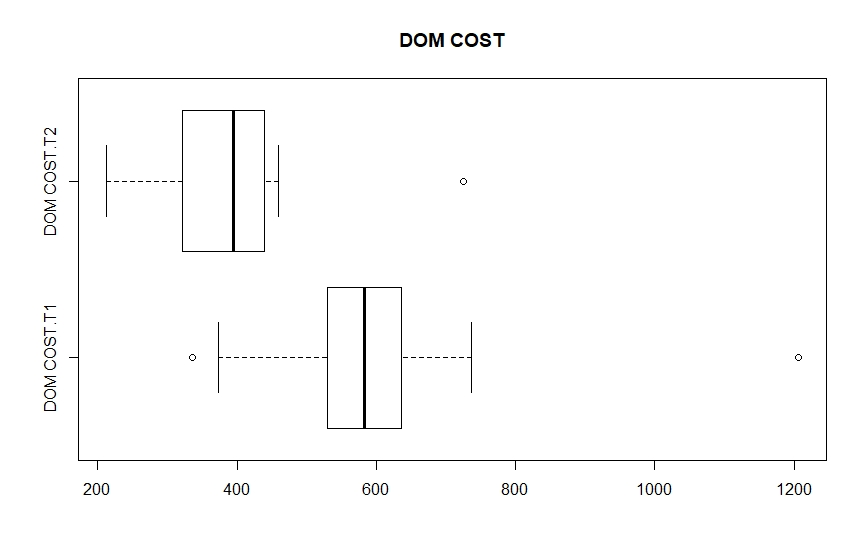
\includegraphics[width=15cm]{RStudio/jpeg/Box DOM.jpeg}
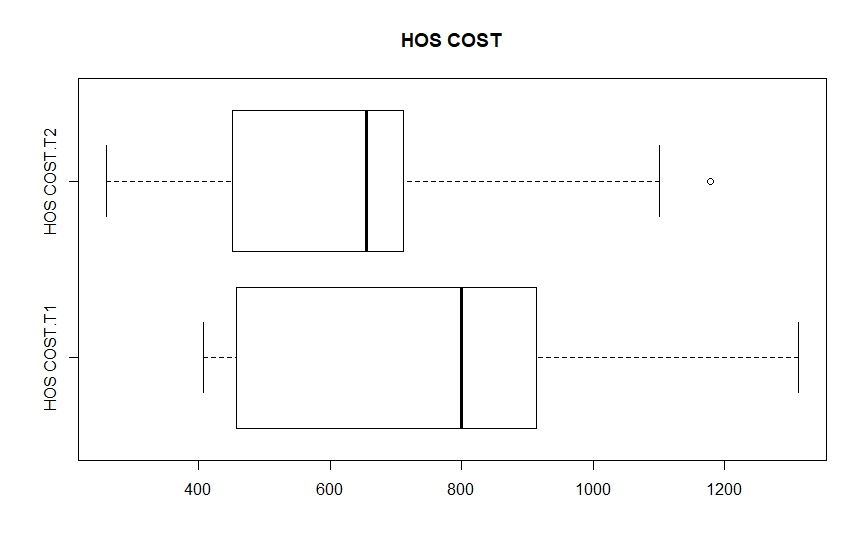
\includegraphics[width=15cm]{RStudio/jpeg/Box HOS.jpeg}
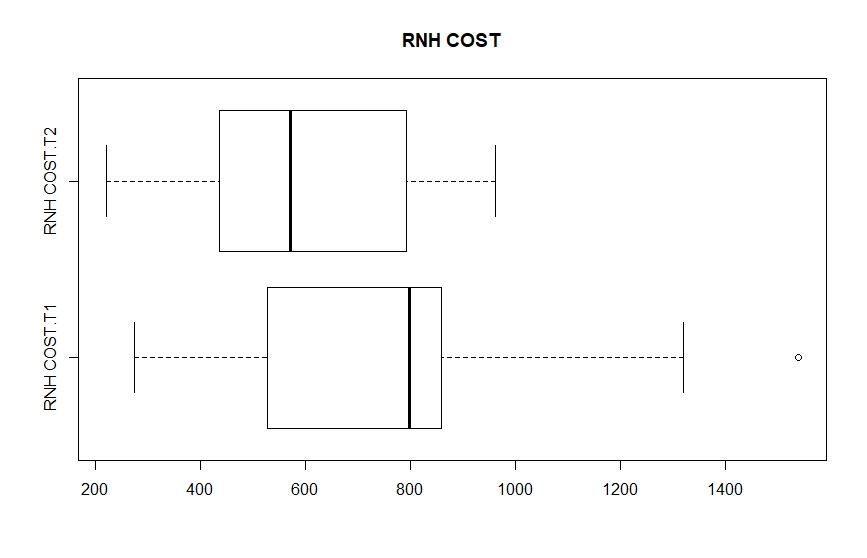
\includegraphics[width=15cm]{RStudio/jpeg/Box RNH.jpeg}
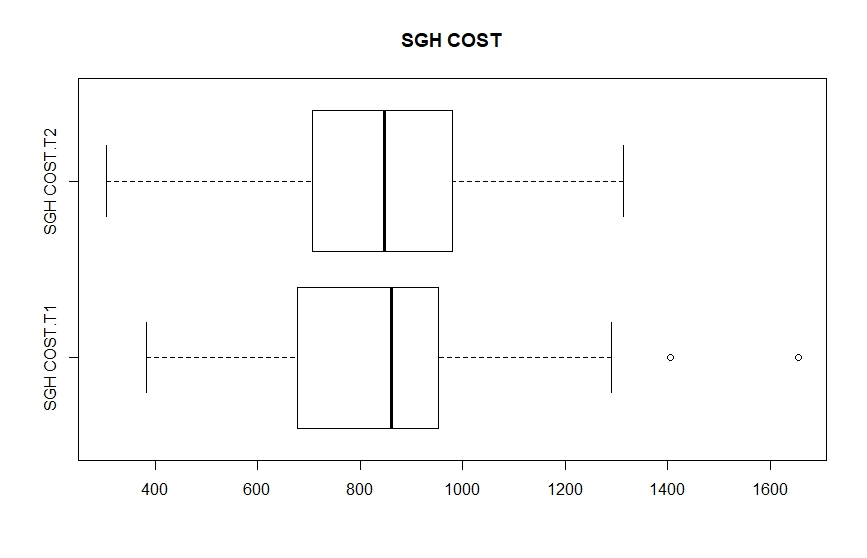
\includegraphics[width=15cm]{RStudio/jpeg/Box SGH.jpeg}
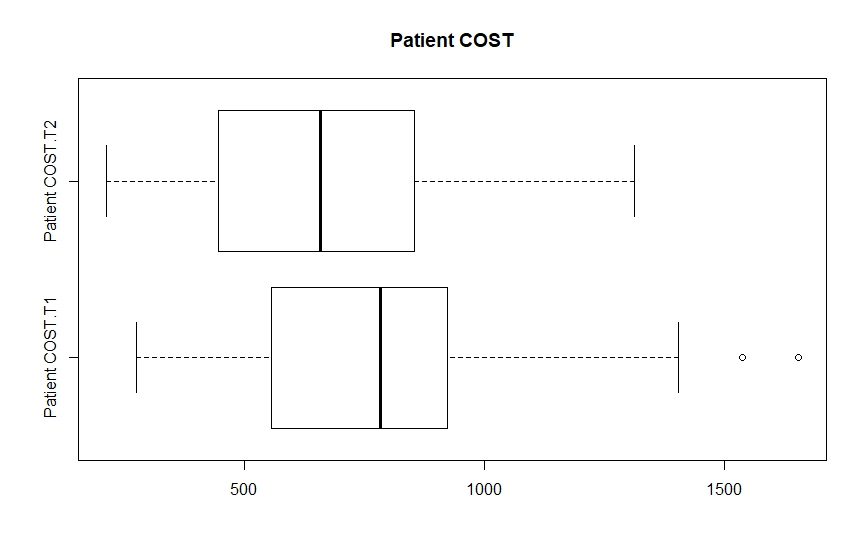
\includegraphics[width=15cm]{RStudio/jpeg/Box COST.jpeg}
\section{Assesment of Normality}
\subsection{Stem and Leaf plots}
\verbatiminput{RStudio/txt/Stem-Leaf.txt}
\subsection{Normal Fit}
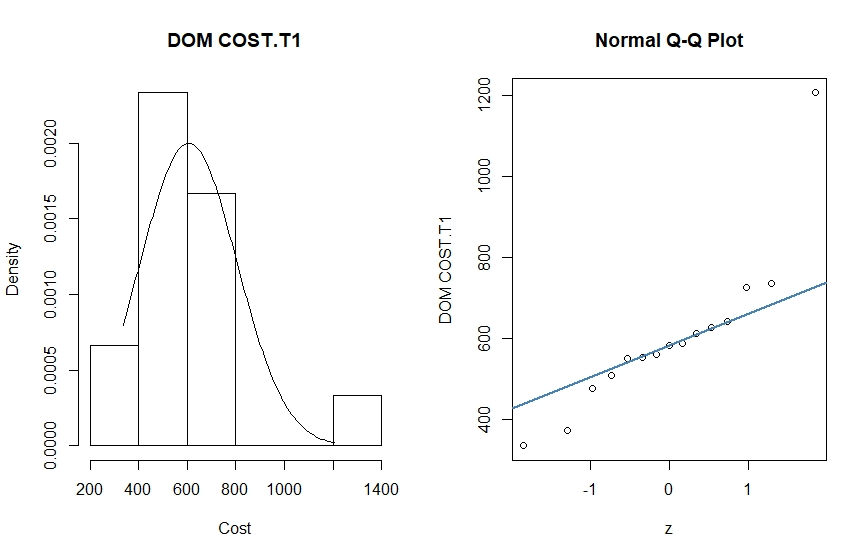
\includegraphics[width=15cm]{RStudio/jpeg/Norm DOM T1.jpeg}
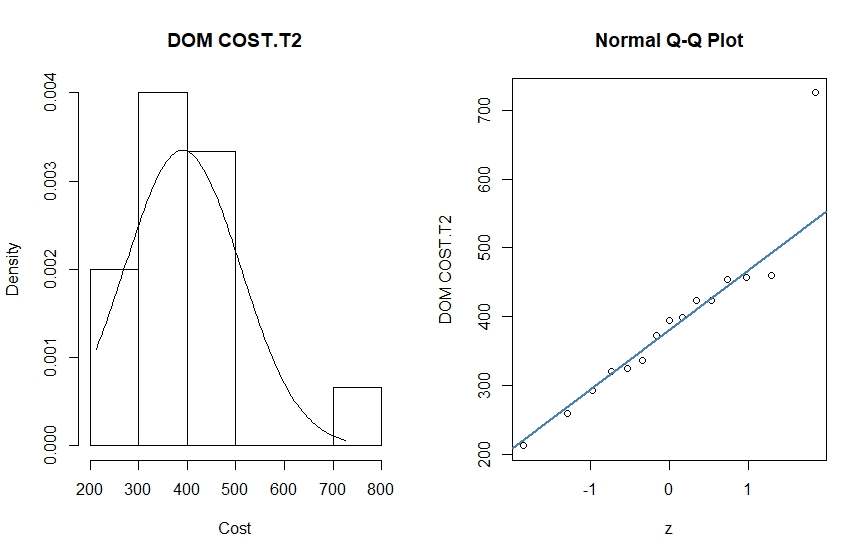
\includegraphics[width=15cm]{RStudio/jpeg/Norm DOM T2.jpeg}

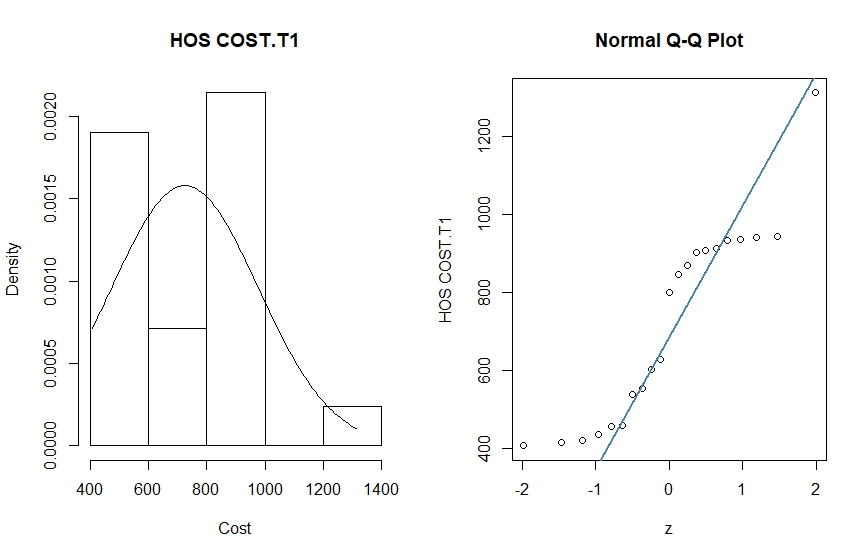
\includegraphics[width=15cm]{RStudio/jpeg/Norm HOS T1.jpeg}
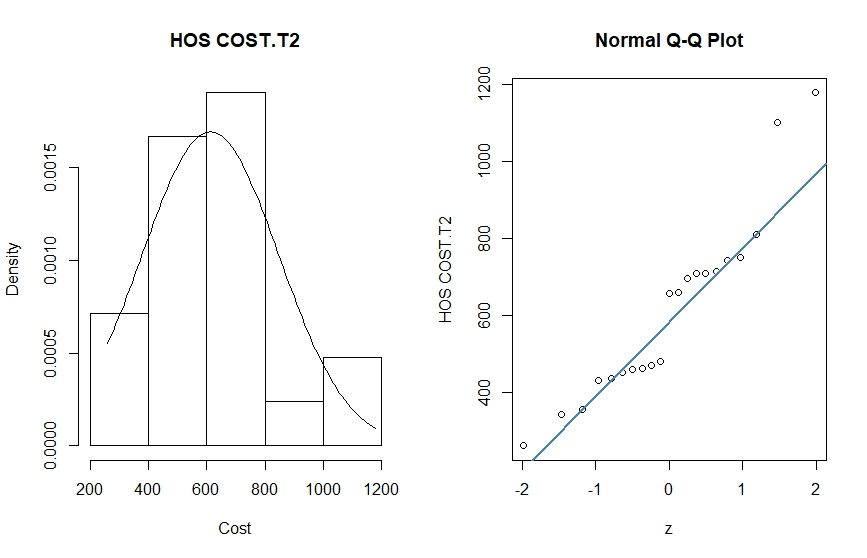
\includegraphics[width=15cm]{RStudio/jpeg/Norm HOS T2.jpeg}

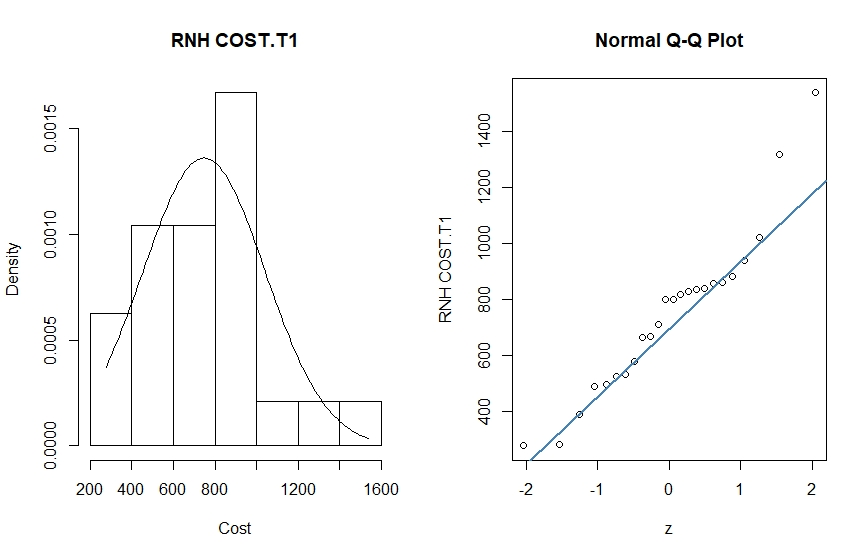
\includegraphics[width=15cm]{RStudio/jpeg/Norm RNH T1.jpeg}
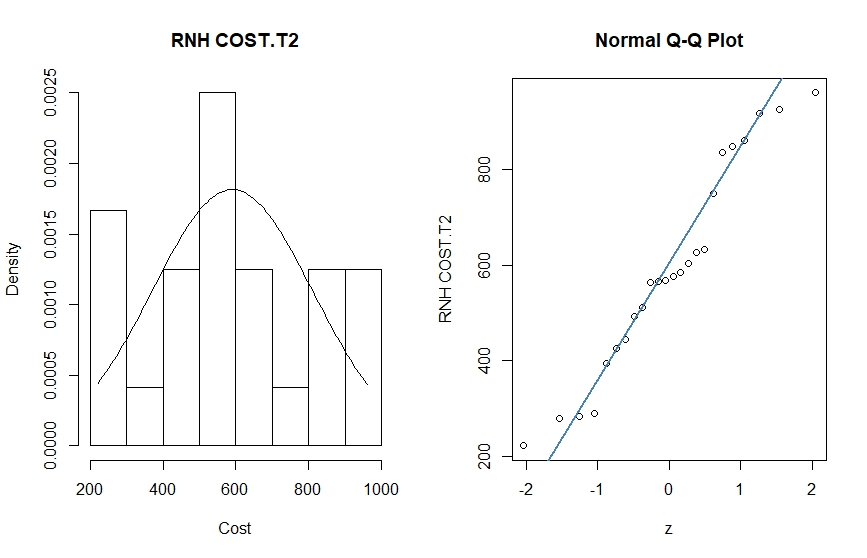
\includegraphics[width=15cm]{RStudio/jpeg/Norm RNH T2.jpeg}

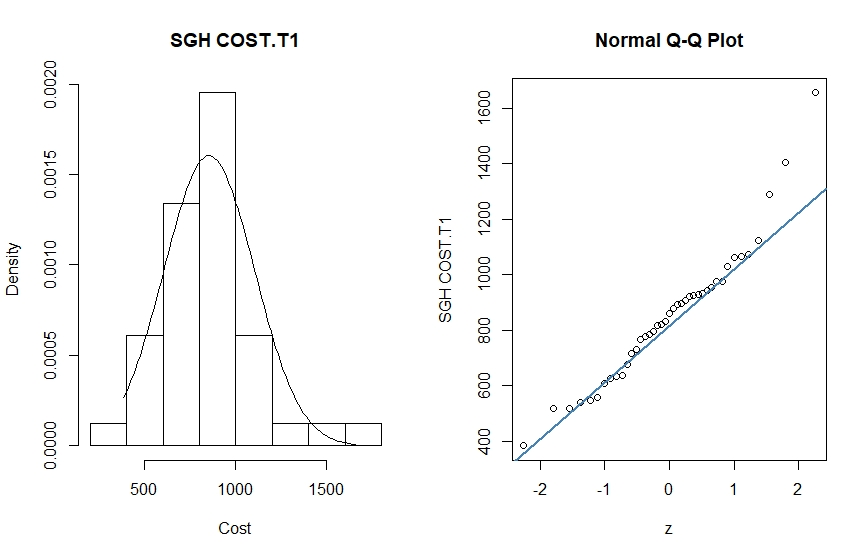
\includegraphics[width=15cm]{RStudio/jpeg/Norm SGH T1.jpeg}
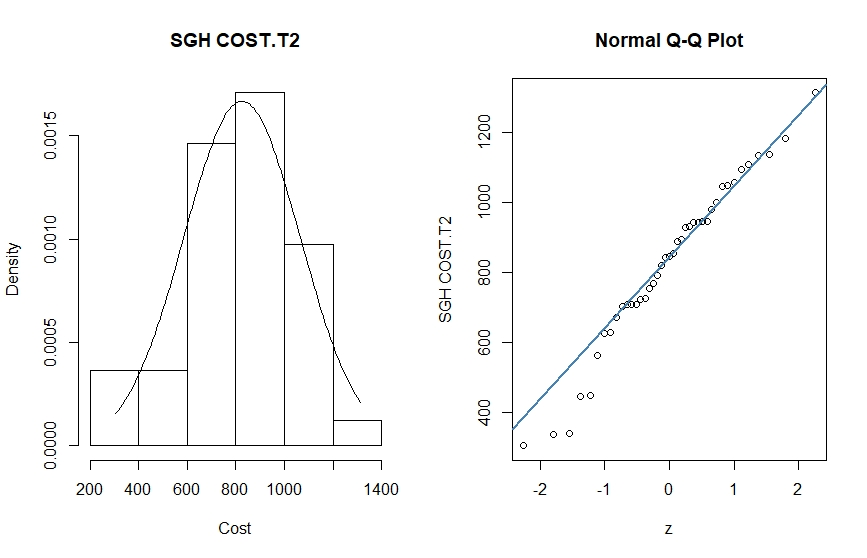
\includegraphics[width=15cm]{RStudio/jpeg/Norm SGH T2.jpeg}

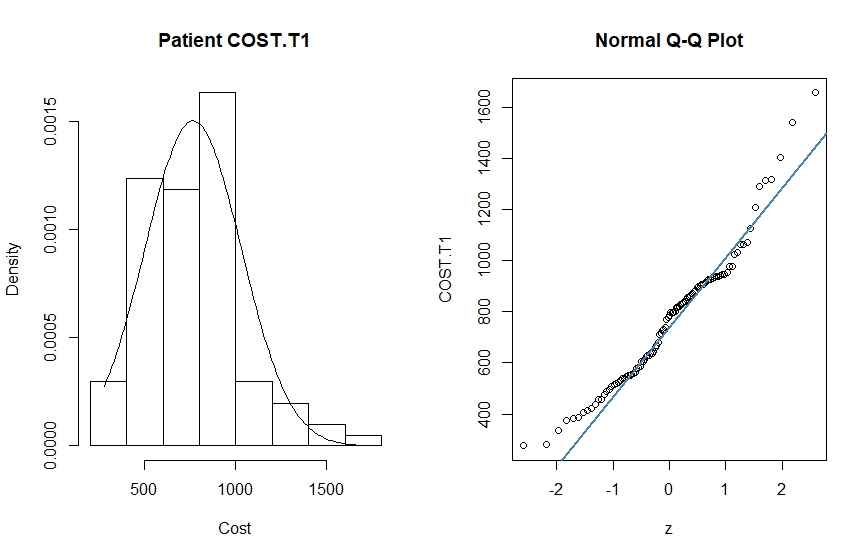
\includegraphics[width=15cm]{RStudio/jpeg/Norm T1.jpeg}
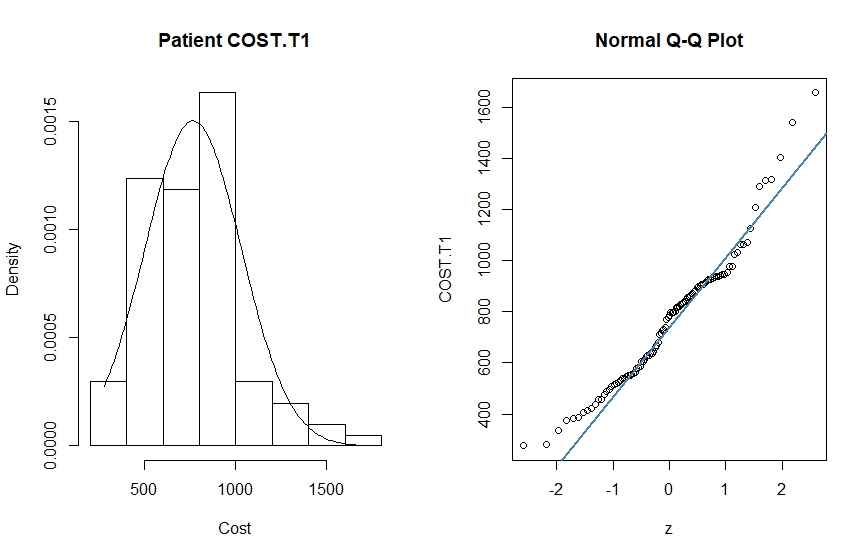
\includegraphics[width=15cm]{RStudio/jpeg/Norm T1.jpeg}


\section{Associations}
\subsection{Linear Models}
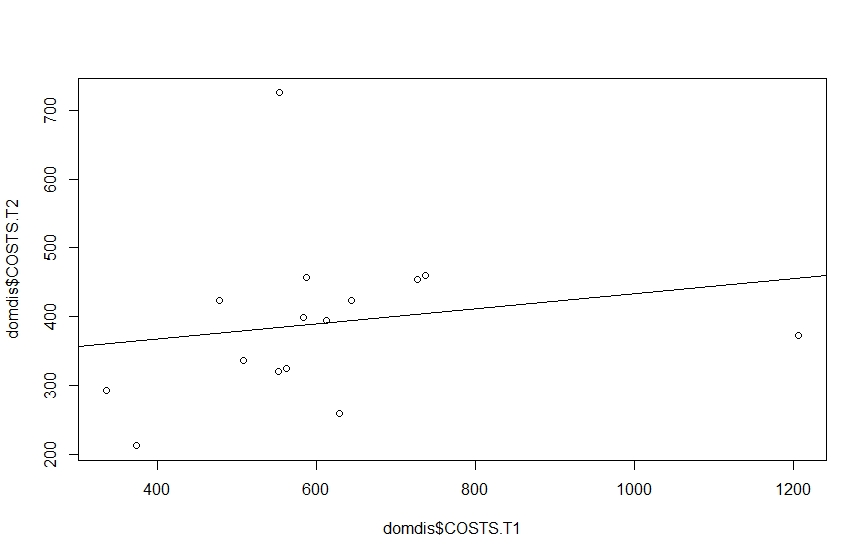
\includegraphics[width=15cm]{RStudio/jpeg/Reg DOM.jpeg}
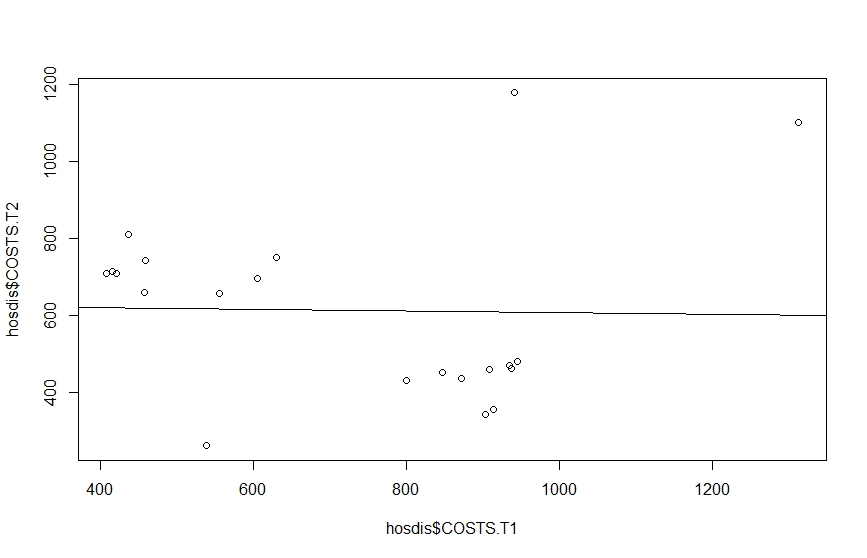
\includegraphics[width=15cm]{RStudio/jpeg/Reg HOS.jpeg}
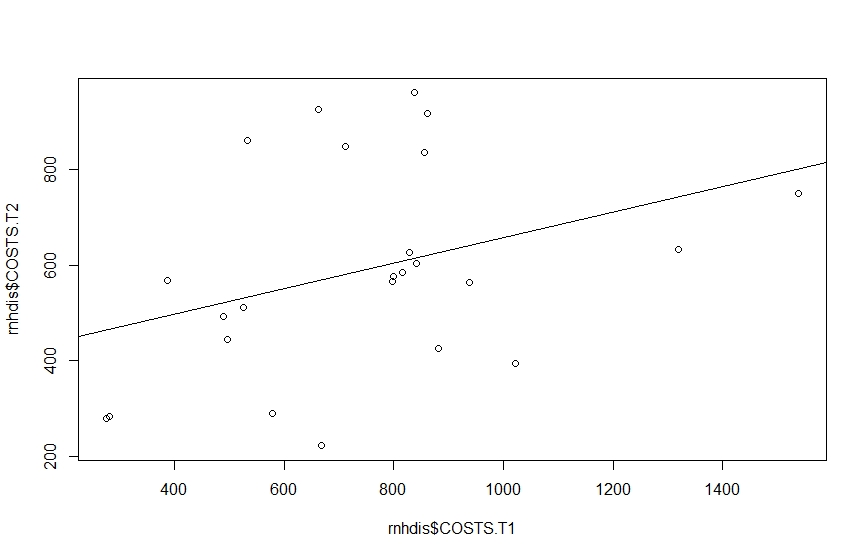
\includegraphics[width=15cm]{RStudio/jpeg/Reg RNH.jpeg}
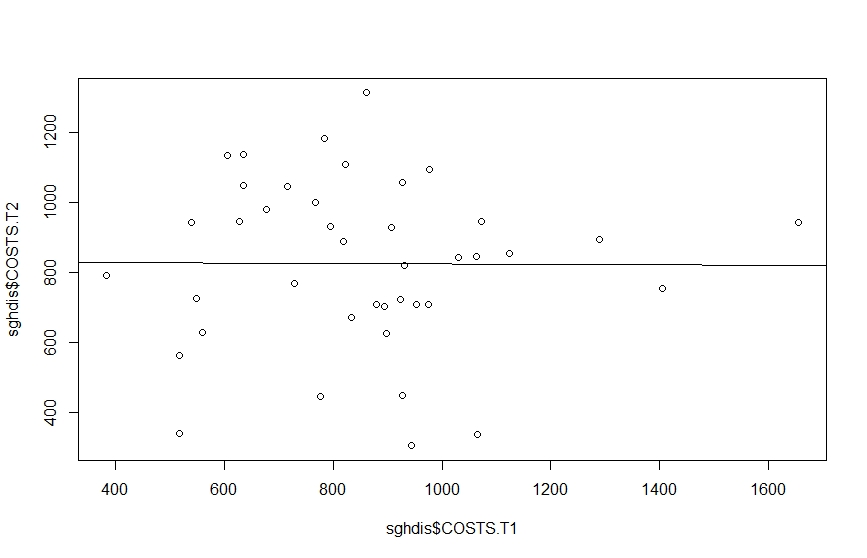
\includegraphics[width=15cm]{RStudio/jpeg/Reg SGH.jpeg}
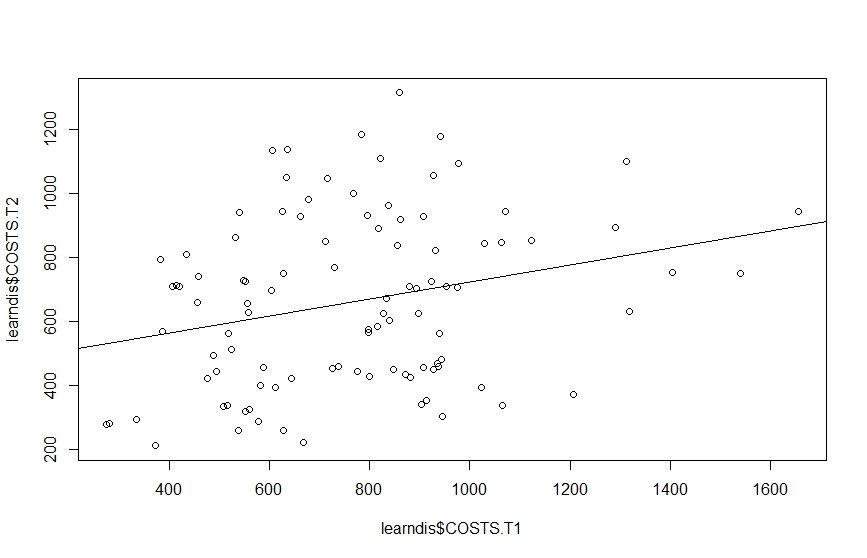
\includegraphics[width=15cm]{RStudio/jpeg/Reg COST.jpeg}

%\verbatiminput{RStudio/txt/Linear-Model-Summaries.txt}
%This throws and error because there is an invalid UTF-8 character
\section{Stability of Associations}

\subsection{Residuals}

\section{Interpretations}

\end{document}

